\documentclass[table]{beamer}
\usepackage{mdwlist}
\usepackage{multirow}
\usepackage{graphicx}
\usepackage{verbatim} % For using /begin{comment}; /end{comment}

% Bright colors
\definecolor{oj}{rgb}{1.0,0.65,0.0}
\definecolor{cblue}{rgb}{0.39,0.58,0.93}
\definecolor{amethyst}{rgb}{0.6, 0.4, 0.8}

% Pale colors
\definecolor{lightgrey}{rgb}{0.75, 0.75, 0.80}
\definecolor{tangerine}{rgb}{1.0, 0.6, 0.4}
\definecolor{arylyellow}{rgb}{0.91, 0.84, 0.42}
\definecolor{gsa}{rgb}{0.66, 0.89, 0.63}
\definecolor{aqua}{rgb}{0.5, 1.0, 0.83}
\definecolor{bblue}{rgb}{0.67, 0.9, 0.93}

\setbeamercolor{normal text}{bg=black, fg=lightgrey}
\setbeamercolor{title}{fg=arylyellow}
\setbeamercolor{frametitle}{fg=tangerine}
\setbeamercolor{framesubtitle}{fg=gsa}
\setbeamercolor{block title}{fg=aqua}
\setbeamercolor{itemize item}{fg=amethyst} % all frames will have red bullets
\setbeamercolor{enumerate item}{fg=amethyst} % all frames will have red bullets
%\setbeamercolor{block title}{fg=green}

\usefonttheme{serif}
\setbeamerfont{frametitle}{series=\bfseries} % Frame titles should be bold

\setbeamertemplate{itemize items}[circle]

\title{\textbf{Coronal Seismology}}
\subtitle{\textbf{ASTR 598}}
\date{\textbf{Spring 2016}}
\author{\textbf{Laurel Farris}}

\begin{document}

{\usebackgroundtemplate{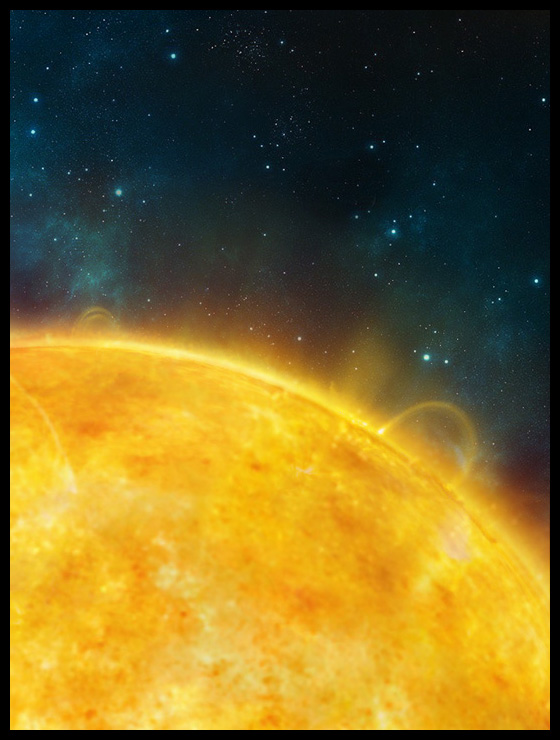
\includegraphics[width=\paperwidth]
    {awesome.jpg}}
\begin{frame}
    \titlepage{}
\end{frame}}%-------------------------------------------------------------%

\begin{frame}{Overview}
    The body of the frame
\end{frame}%-------------------------------------------------------------%

\begin{frame}{Motivation/Main Scientific Question}
    \begin{itemize}
        \item The coronal heating problem
    \end{itemize}
\end{frame}%-------------------------------------------------------------%

\begin{frame}{Basic MHD}{Theory before observations}
    Types of waves/oscillations:
    \begin{itemize*}
        \item Alfv\'en: $V_A = \frac{B}{\mu_0\rho}$
        \item Magnetoacoustic: $C_s = \sqrt{\frac{\gamma P}{\rho}}$
            \begin{itemize*}
                \item Fast $C_{A_0} < C_{fast} < C_{A_e} $
                \item Slow $C_{T_0} < C_{slow} < C_{s_0} $
            \end{itemize*}
    \end{itemize*}
\end{frame}%-------------------------------------------------------------%

\begin{frame}
    \begin{figure}
        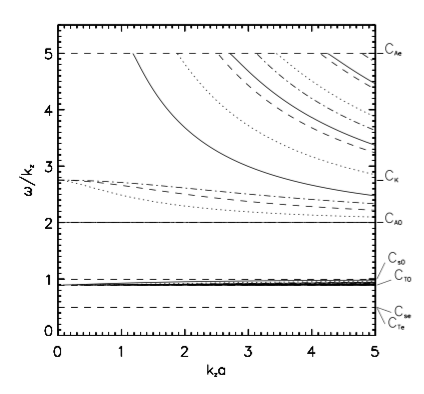
\includegraphics[width=3in]{disp_diagram.png}
    \end{figure}
\end{frame}%-------------------------------------------------------------%

\begin{frame}{MHD equations}
$ \xi(x) = \xi(r)e^{i(kz+m\phi)}  $
\end{frame}%-------------------------------------------------------------%

\begin{frame}{MHD modes}
    \begin{itemize}
        \item Kink
        \item Sausage
        \item Acoustic
        \item Propagating acoustic modes
        \item Propagating fast modes
        \item Torsional modes (aka.\ Alfv\'en waves)
    \end{itemize}
\end{frame}%-------------------------------------------------------------%
\begin{frame}{Kinks vs.\ Sausages}
%\begin{center}
\begin{columns}
        \column{0.6\textwidth}
    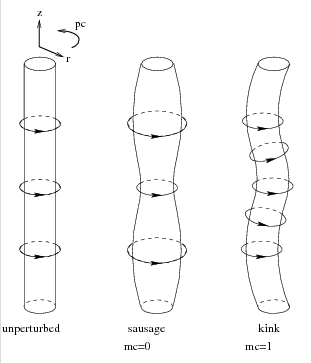
\includegraphics[width=2.5in]{kink_saus.png}
    %\par{\tiny image credit:\\
    %$https://inspirehep.net/record/1088737/files/figures_instab_locations.png$}
    %\end{center}
        \column{0.4\textwidth}
    \begin{block}{Kink}
        \begin{itemize}
            \item loop spatial displacement
            \item Asymmetric
            \item No intensity change
            \item $k\sigma \ll 1$, or $\sigma\ll\lambda$
        \end{itemize}
    \end{block}
    \begin{block}{Sausage}
        \begin{itemize}
            \item No loop spatial displacement
            \item Symmetric
            \item Intensity change\\ $\rightarrow$ density change
            \item $\lambda\sim\sigma$
        \end{itemize}
    \end{block}
\end{columns}
\end{frame}%-------------------------------------------------------------%
\begin{frame}{Kink modes}
{Coronal loop oscillations observed with the
\emph{Transition Region And Coronal Explorer (TRACE)}}
    \begin{itemize}
        \item Gaussian vs.\ exponential
        \item Plasma motions around footpoints of coronal loops
    \end{itemize}
\end{frame}%-------------------------------------------------------------%
\begin{frame}{Kink modes}{Excitation and damping of broadband kink waves
    in the solar corona}
\end{frame}%-------------------------------------------------------------%
\begin{frame}{Sausage modes}{Observations of sausage modes in magnetic pores}
\end{frame}%-------------------------------------------------------------%
\begin{frame}{Sausage modes}{Sausage waves in transversely nonuniform
    monolithic coronal tubes}
\end{frame}%-------------------------------------------------------------%
\begin{frame}{Acoustic oscillations}
\end{frame}%-------------------------------------------------------------%
\begin{frame}{Propagating acoustic waves}
    Nodes are in motion; \emph{traveling waves}
    (Oscillations have fixed nodes).
\end{frame}%-------------------------------------------------------------%
\begin{frame}{Propagating fast waves}
    \begin{itemize}
        \item Moreton waves in the chromosphere
        \item Fast EUV waves in the corona
    \end{itemize}
\end{frame}%-------------------------------------------------------------%
\begin{frame}{Torsional modes}{aka.\ Alfv\'en wave}
\end{frame}%-------------------------------------------------------------%
\begin{frame}{Mixed modes}{Pulling individual modes out}
\end{frame}%-------------------------------------------------------------%
\begin{frame}{Important Properties}
    \begin{center}
        \begin{tabular}{c|c|c|c|}
            \cline{2-4} & \textbf{timescale} & \textbf{sizescale} &
                \textbf{obs.\ method}\\
            \hline \multicolumn{0}{|c|}{kink osc} & value & value & value\\
            \hline \multicolumn{0}{|c|}{sausage osc} & value & value & value\\
            \hline \multicolumn{0}{|c|}{acoustic osc} & value & value & value\\
            \hline \multicolumn{0}{|c|}{acoustic waves} & value & value & value\\
            \hline \multicolumn{0}{|c|}{fast waves} & value & value & value\\
            \hline \multicolumn{0}{|c|}{torsional modes} & value & value & value\\
            \hline \multicolumn{0}{|c|}{mixed modes} & value & value & value\\
            \hline
        \end{tabular}
    \end{center}
\end{frame}%-------------------------------------------------------------%
\begin{frame}{Example Table}
\begin{center}
   \begin{tabular}{cc|c|c|}
% row 1
   \cline{3-4} & & \multicolumn{2}{|c|}{Condition (Gold standard)}\\
% row 2
   \cline{3-4} & & True & False \\
   \hline
% row 3 (and 4) - multirow
   \multicolumn{1}{|c|} % add in vertical lines
   {\multirow{2}{*}{Test outcome}}& % Text covers rows 3 and 4
 % row 3
   \multicolumn{1}{|c|}{Positive} %
     & True Positive \cellcolor{green} & False Positive\cellcolor{red}\\
 % row 4
   \cline{2-4} \multicolumn{1}{|c|}{}
     & \multicolumn{1}{|c|}{Negative}
     & False Negative\cellcolor{red} & True Negative \cellcolor{green}\\
    \hline
    \end{tabular}
\end{center}
\end{frame}%-------------------------------------------------------------%

\begin{frame}{Example of Two Column Output}
    \begin{columns}[c]
        \column{1.5in}
            Practical \TeX\ 2005\\
            Practical \TeX\ 2005\\
            Practical \TeX\ 2005
        \column{1.5in}
            % put nice little frame around graphic
            \framebox{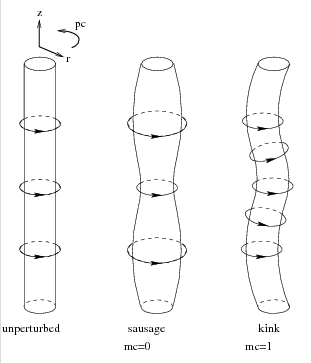
\includegraphics[width=1.5in]{kink_saus.png}}
    \end{columns}
\end{frame}%-------------------------------------------------------------%


\begin{frame}{My Research}
\end{frame}%-------------------------------------------------------------%

\end{document}
